\documentclass{article}

\usepackage[utf8]{inputenc} 
\usepackage{outlines}
\usepackage{amsmath}
\usepackage{cleveref}
\usepackage{graphicx}
\usepackage{xr}

\usepackage[margin=1in]{geometry}
\parskip 1.5ex % paragraph spacing

\graphicspath{./docs/Figures/}

\title{Temp RM}
\author{Tom}
\date{January 2021}

\begin{document}

\maketitle

\section{Introduction}

Temperature has long been recognised as a fundamental environmental driver in ecology, affecting many aspects of the structure (REF) and function (REF) of ecological systems. Understanding the mechanisms that underlie these effects is important given the ubiquity of temperature gradients across space (e.g. latitudinal or elevations gradients) and time (e.g. seasonal fluctuations) and the potential of temperature's influence to be felt across multiple scales of organisation, from individual physiological rates (REF) to community and ecosystem dynamics (REF). In addition to these processes shaping natural systems temperature is becoming increasingly relevant to modern ecology given accelerating rates of global warming, with the IPCC predicting ~X increase in global temperature over the next 50 years. 


One aspect of temperature that is of particular interest is how it affects ecosystem dynamics, the changes in distributions of biomass over time. 

How temperature affects the dynamics of ecosystems, the changes in biomass over time, is of particular interest to ecologists given both the  . Though empirical work has shown that temperature has effects on communities and thier structure and dynamics little work has been done to understand a mechanistic understanidn g fo therses effects. This stands in contrast to many other ares of ecology where MTE has been applied to understand how temperature affects various ecological processes. 

Here we examine how temperature affects the feasibility of ecosystems. An ecosystem is feasabile if all sepcies have positive biomass. feasabiltiy is an important and often ignoreed aspect of ecosystem dynamics, often relegated to an assumption in classic stablitiy stuff. Recent worj has demonstrated that the feasbiltiy of ecosystems arrises from the interplay of specieis intrisigc growth rates and the nature ans structure of thoer interactions. It follows that temperature should affect these aspects give how it affects these compoentnet

In addition to underlying ecosystem dynamics feasability is also important as a driver 



\section{Theory}
\subsection{Model}
In order to explore feasibility and its temperature dependence we use the generalised Lottka-Volterra model (GLV) (REF). This framework is commonly used to explore ecosystem dynamic properties and is regularly applied to study complex, multi-species communities (REF). The GLV describes the dynamics of an $N$ species system where the growth of species $i$ is given by:

\begin{equation} \label{EQ:GLV}
  \frac{1}{x_i} \frac{dx_i}{dt} = r_i - a_{ii} x_i - \sum^N_{i \neq j} a_{ij} x_j, 
\end{equation}

where $x_i$ is the biomass of the $i$th species, $r_i$ is it's intrinsic growth rate, determining the rate at which new biomass is produced ($\text{mass} \cdot \text{time}^{-1} \cdot \text{mass}^{-1} $) and $a_{ij}$ describes the effect of interactions with species $j$ on $i$ (with the $a_{ii}$ term representing intraspecific interactions; $\text{mass}^{-1} \cdot \text{time}^{-1}$). As we want to determine the feasibility of this system (i.e. whether the system will support non-zero biomasses for all species at equilibrium) we need to derive an expression for the equilibrium biomasses. Though it is not possible to derive an exact analytical solution for the GLV as described in \cref{EQ:GLV}, we can use a mean-field approximation, developed by (REF) to get estimate of equilibrium biomass (\cref{SI_Sec:Meanfield}). This approximation works by considering interaction term from \cref{EQ:GLV}, which we can rewrite as:

\begin{equation} \label{EQ:mean_int} 
    \sum^N_{i \neq j} a_{ij} x_j = (N-1) \bar{a x} = (N-1) \bar{a} \bar{x} + (N-1) \text{cov}(a,c),
\end{equation}

where the bar notation, $\bar{\cdot}$, represents the average of that quantity over all $N$ species in the system. \Cref{EQ:mean_int} partitions the effects of interactions on the $i$th species into the average effect across the system, $\bar{a} \bar{x}$, and the covariance between heterospecific's biomass and the strength of interactions, $\text{cov}(a,x)$. The mean-field approximation assumes that this second term is negligible, which is equivalent to saying that any individual interaction between the focal species and another species population has little effect on that heterospecific's biomass. We also assume here that the system we consider is large ($N \gg 0$), meaning that the difference between the average biomass across the system and that of heterospecifics is small (as it is in the order $N^{-1}$) and can thus be ignored. We also make the further assumption for simplicity that intraspecific interactions are constant across species, setting $a_{ii} = 1$. Combining \cref{EQ:GLV,EQ:mean_int}  we can then express population dynamics in terms the average interaction strength, giving the full mean-field model:

\begin{equation} \label{EQ:MF}
    \frac{1}{x_i} \frac{dx_i}{dt} \approx r_i - x_i - (N-1)\bar{a}\bar{x}.
\end{equation}

By setting \cref{EQ:MF} equal to $0$ and solving for $x_i$ we then obtain an expression for equilibrium biomass (see \cref{SI_Sec:Meanfield}):

\begin{equation}\label{EQ:MF_eqi}
  x^*_i \approx K_i -  \bar{K}  \frac{ (N-1)\bar{a}}{1 + (N-1)\bar{a}}, 
\end{equation}

where $K_i = \frac{r_i}{a_{ii}}$ is the carrying capacity, the biomass a population would reach if grown in isolation (obtained by solving \cref{EQ:MF} with $\bar{a} = 0$). \Cref{EQ:MF_eqi} provides an intuitive expression for the equilibrium biomasses; a species is expected to reach the biomass that it would in isolation (first term of the RHS, $K_i$) minus the effects of any interspecific interactions (second term on RHS). The strength of these interspecific effects is determined by the average biomass heterospecifics would reach ($\bar{K}$) and a saturating function of interactions experienced by the focal species, $(N-1)\bar{a}$. If interactions are overall competitive (i.e. $ \bar{a} > 0$) then we see a reduction in equilibrium biomass relative to the individual carrying capacities whereas if they are facilitatory ($ \bar{a} < 0$) we see an increase.  

\subsection{Feasibility} \label{Sec:Feasibility}
We use \Cref{EQ:MF_eqi} to derive an expression for the feasibility of a system in terms of the population demographic parameters (i.e. the $r_i$'s and $a_{ij}$'s). We start by recalling that a system is feasible if all species have non-zero equilibrium biomass (i.e. $x_i^* > 0 $), giving the condition:

\begin{align} \label{EQ:Feas_sp}
  \kappa_i > \frac{(N-1)\bar{a}}{1 + (N-1)\bar{a}} \quad \text{for all} \quad i = 1 \ldots N,
\end{align}

where $\kappa_i = \frac{K_i}{\bar{K}}$ is the mean-normalised carrying capacity. \Cref{EQ:Feas_sp} shows how a system is feasible as long as the the negative effects of interspecific interactions on the each population (RHS) do not outweigh the effects of intraspecific interactions (LHS). We test this prediction using numerical simulations of randomly generated GLV communities (which vary in their values of normalised carrying-capacity $\kappa$ and interaction strength), showing the analytical condition predicts the feasibility of systems well (\cref{Fig:Feasability_Bound}; \cref{SI_Sec:Feas_sims}). 

\begin{figure}[h] 
    \centering
    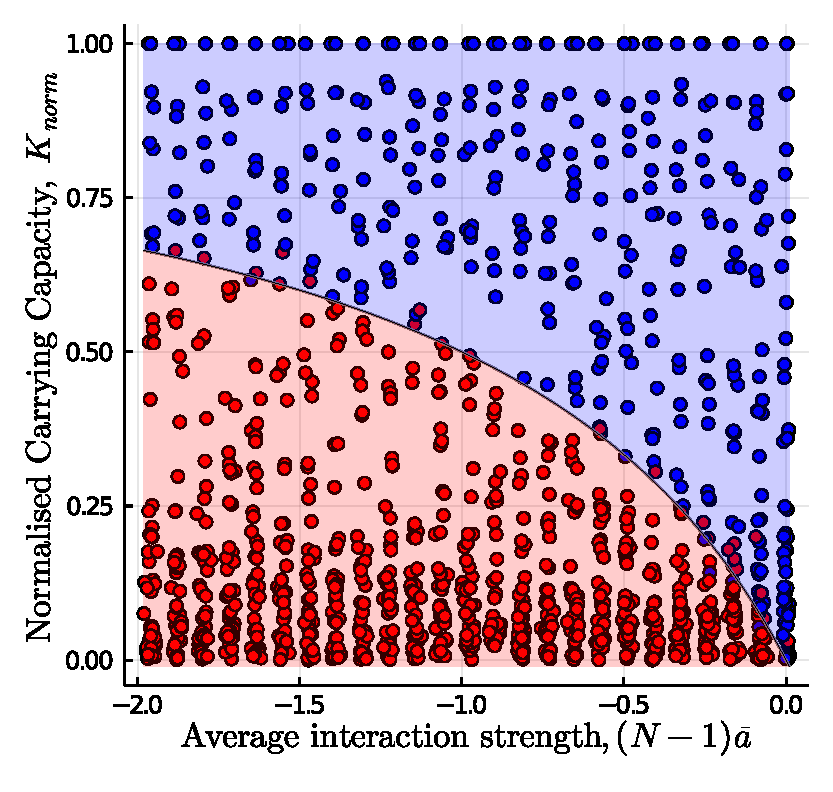
\includegraphics[width = 0.5\textwidth]{docs/Figures/Fig_1.pdf}
    \caption[width = \textwidth]{\textbf{Analytical predictions of feasibility} The bound given by \cref{EQ:Feas_sp} predicts feasibility in randomly generated GLV communities. The theoretical bound (black line) gives the minimum value for $\kappa$ below which (area shaded in red) communities are unfeasible (i.e extinctions have occurred) and above which (shaded blue) communities are feasible. Each point shown is the minimum $\kappa$ value from a randomly generated community with $N=50$ simulated till equilibrium. Feasible systems (with no extinctions) are shown in blue and unfeasible systems in red.}
    \label{Fig:Feasability_Bound}
\end{figure}

Using \cref{EQ:Feas_sp} we can also formulate an expression for the probability of feasibility $P_{feas}$, the chance that an ecosystem is feasible given the distribution of species trait values ($\kappa$s and $a$s) and number of species in the system. To do so we take \cref{EQ:Feas_sp} and consider $\kappa$ and $a$ as random variables, each describing the distribution of the respective traits across the community (represented in notation by the loss of subscript). In doing so we can consider $\kappa$'s cumulative density function (CDF) which gives the probability that $\kappa$ is less than or equal to some value, $F_{\kappa}(x) = P(\kappa \leq x)$. As the condition for feasibility states that $\kappa$ must be greater than the effect of interactions we can apply the CDF to \cref{EQ:Feas_sp} and write $P_{feas}$ as:

\begin{equation} \label{EQ:P_feas}
    P_{feas} = P \left( \kappa > \frac{(N-1)\bar{a}}{1 + (N-1)\bar{a}}  \right)^N = 
    \left[1 - F_{\kappa}\left(\frac{(N-1)\bar{a}}{1 + (N-1)\bar{a}}\right)\right]^N
\end{equation}

thus giving the probability of feasibility as a function of the species traits (\cref{Fig:P_feas}). Note the expression is raised to the $N$th power as the term in the brackets must hold for all $N$ populations in the system for it to be feasible. 

\begin{figure}
    \centering
    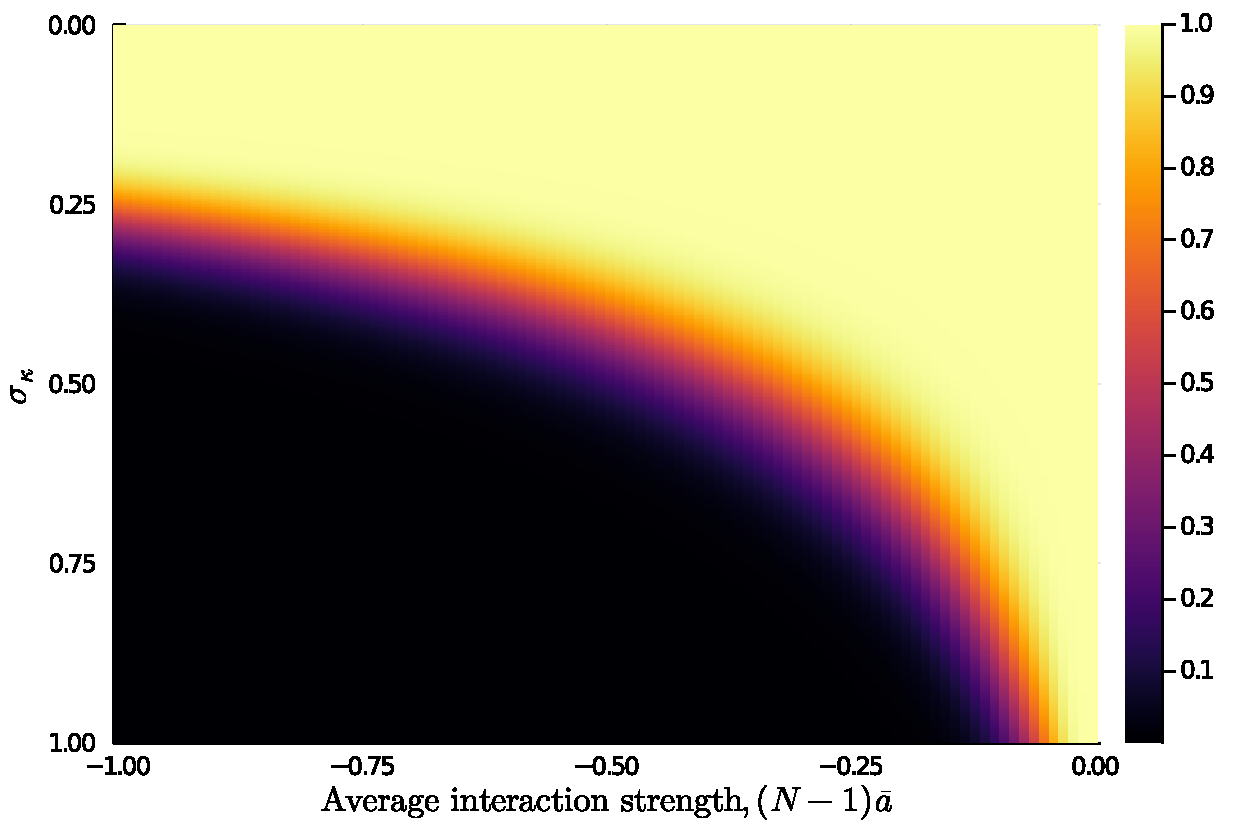
\includegraphics[width = 0.6\textwidth]{docs/Figures/Fig_2.pdf}
    \caption{\textbf{The probability of feasibility $P_{feas}$ as a function of interaction strength and variation in normalised carrying capacity $\sigma_{\kappa}$}. Feasibility shows the same general pattern as \cref{Fig:Feasability_Bound}, decreasing as interactions become more negative and as the variation in $\kappa$ increases (reducing the chance that all species meet the criteria in \cref{EQ:Feas_sp}). $P_{feas}$ is calculated using \cref{EQ:P_feas} setting $N=50$ and allowing $\sigms_{\kappa}$ and $\bar{a}$ to vary such that $\sigma_{\kappa} \in [0 - 1]$ and $\bar{a} \in [-1 - 0]$}
    \label{Fig:P_feas}
\end{figure}

\subsection{Temperature} \label{SEC:Temperature}
In order to relate the conditions for feasibility discussed in \cref{Sec:Feasibility} to temperature we next consider how temperature affects the parameters determining feasibility in \cref{EQ:P_feas}, the normalised carrying capacities $\kappa$ (driven here primarily by changes in population growth rate $r$), and inter-species interactions $a$. There is a large body of empirical and theoretical work demonstrating the existence and consequences of the temperature dependence of these processes, which can be explained by their dependence on metabolic rate (which determines the capacity of individuals to fuel growth and interactions), which in turn is affected by temperature through its effects on biochemical kinetics (REF).

We use the modified Boltzmann-Arrhenius equation to represent the thermal dependence of $\kappa$ and $a$ which describes the exponential-like increase of some process $B(T)$ with temperature (REF). Though empirically measured temperature response curves tend to show a uni-modal shape, we use the Boltzmann-Arrhenius due to both its analytic tractability and its ability to capture the rising portion (before the temperature peak) of these curves. We focus on this part of the curve as it is expected that the range of temperatures individuals actually experience (their operational temperature range) tends to below this thermal peak, making the exponential portion more relevant for the dynamics of real ecosystems (REF). This form of the Boltzmann-Arrhenius uses two parameters to describe the thermal response of a given process, the normalisation constant $B_0$ which is the value at a reference temperature and thermal sensitivity $E$ which determines the magnitude of the response of $B(T)$ to changes in temperature and has the form:

\begin{equation} \label{EQ:Boltzmann}
    B(T) = B_0 e^{-\frac{E}{k} \left(\frac{1}{kT} - \frac{1}{k T_{ref} }\right)},
\end{equation}

where $k$ is the Boltzmann constant and $T$ and $T_{ref}$ are the temperature and reference temperature (in kelvin) respectively. 

In order to apply this to our measure of feasibility in \cref{EQ:P_feas} we consider how the values of $B_0$ and $E$ for both $\kappa$ and $a$ are distributed across populations in the ecosystem. We then use these distributions and \cref{EQ:Boltzmann} to determine the actual distribution of parameters values across populations at a given temperature. This in is used to calculate the probability of feasibility as per \cref{EQ:P_feas} (\cref{SI_Sec:TPC_dist}). Assuming that the distribution of parameter values across species follows a log-normal distribution (a natural assumption given the exponential form of \cref{EQ:Boltzmann}) we obtain an expression for the temperature dependent distribution of $B(T)$ (\cref{SI_Sec:TPC_dist}):

\begin{align} \label{EQ:Boltz_dist}
    \log(B(T)) \sim \mathcal{N}\left(\mu_{B}(T) , \sigma_{B}^2(T) \right) 
    \quad \text{where} \quad
    \begin{array}{cc}
        \mu_B &= \mu_{B_0} - \mu_{E} \left(\frac{1}{kT} - \frac{1}{k T_{ref} }\right)  \\
        \sigma_{B}(T)^2 &= \sigma_{B_0}^2 + \sigma_{E}^2 \left(\frac{1}{kT} - \frac{1}{k T_{ref} }\right)^2
    \end{array}
\end{align}

where $\mu$ and $\sigma^2$ represent the mean and variance respectively. Of particular interest in \cref{EQ:Boltz_dist} is the effect of the distribution of thermal sensitivities, $E$, on the realised distribution of $B(T)$. From \cref{EQ:Boltz_dist} we can see that in log-scale the average value of $B(T)$ is a linear function of temperature, the slope of which is determined by the average thermal sensitivity $\mu_E$. The variance however is quadratic, with a minimum at $T = T_{ref}$. This means that when we consider the distribution in linear space (by taking the exponent)  creating uni-modality in the realised distribution of $B(T)$. Applying \cref{EQ:Boltz_dist} to the distributions of $\kappa$ and $\bar{a}$ we obtain the expressions

\begin{align} \label{EQ:Trait_distributions}
    \begin{array}{cc}
        \log(\kappa(T)) &\sim \mathcal{N}\left( -\frac{\sigma_{K}^2(T)}{2} , \sigma_{K}^2(T) \right) \\ \\
        \bar{a}(T) &= \exp \left(\mu_a(T) + \frac{\sigma_a^2(T))}{2} \right)
    \end{array}
\end{align}

which show how these two parameters change with temperature. Crucially we see that the uni-modality which arises from the variance terms will enter both the distribution of normalised carrying capacity $\kappa$ and average interaction strength $\bar{a}(T)$. Combining these with \cref{EQ:Feas_sp,EQ:P_feas} we can write the probability of feasibility directly as a function of temperature:

\begin{equation} \label{EQ:P_feas_Temp}
    P_{feas}(T) = \left[1 - F_{\kappa}\left(T , \frac{(N-1)\bar{a}(T)}{(N-1)\bar{a}(T) + 1} \right) \right]^N.
\end{equation}

Making explicit the relationship between temperature and the feasibility of complex ecosystems. 

\subsection{Species Richness} \label{SEC:N_Sp}
Having defined the relationship between feasibility and temperature we now turn to the question of species richness. From \cref{EQ:P_feas_Temp} we can see that the number of species in an ecological community $N$ can alter its feasibility through two mechanisms. Firstly it alters the strength of interactions experienced by individual populations via the $(N-1) \bar{a}$ term. This will reduce or increase the probability of feasibility depending on the strength of $\bar{a}$. Secondly, the probability of feasibility falls as the number of species increases as it becomes less likely that all $N$ species meet the criteria in \cref{EQ:Feas_sp}. This relationship is represented in the power term in \cref{EQ:P_feas_Temp}. 

In order to explore this relationship and the influence of temperature we take \cref{EQ:P_feas_Temp} and ask at a given temperature what is the maximum number of species an community can support and stay above a given probability of feasibility? Though ideally one would do this by taking \cref{EQ:P_feas_Temp} and solving for $N$ this is not possible for most distributions of $\kappa$ due to the complexity of their cumulative density functions. Instead we numerically solve \cref{EQ:P_feas_Temp} (REF) for $N$ across a range of temperatures allowing us to look at species richness as a function of temperature and the influence of distributions in thermal response parameters across the community. 

\begin{figure}
    \centering
    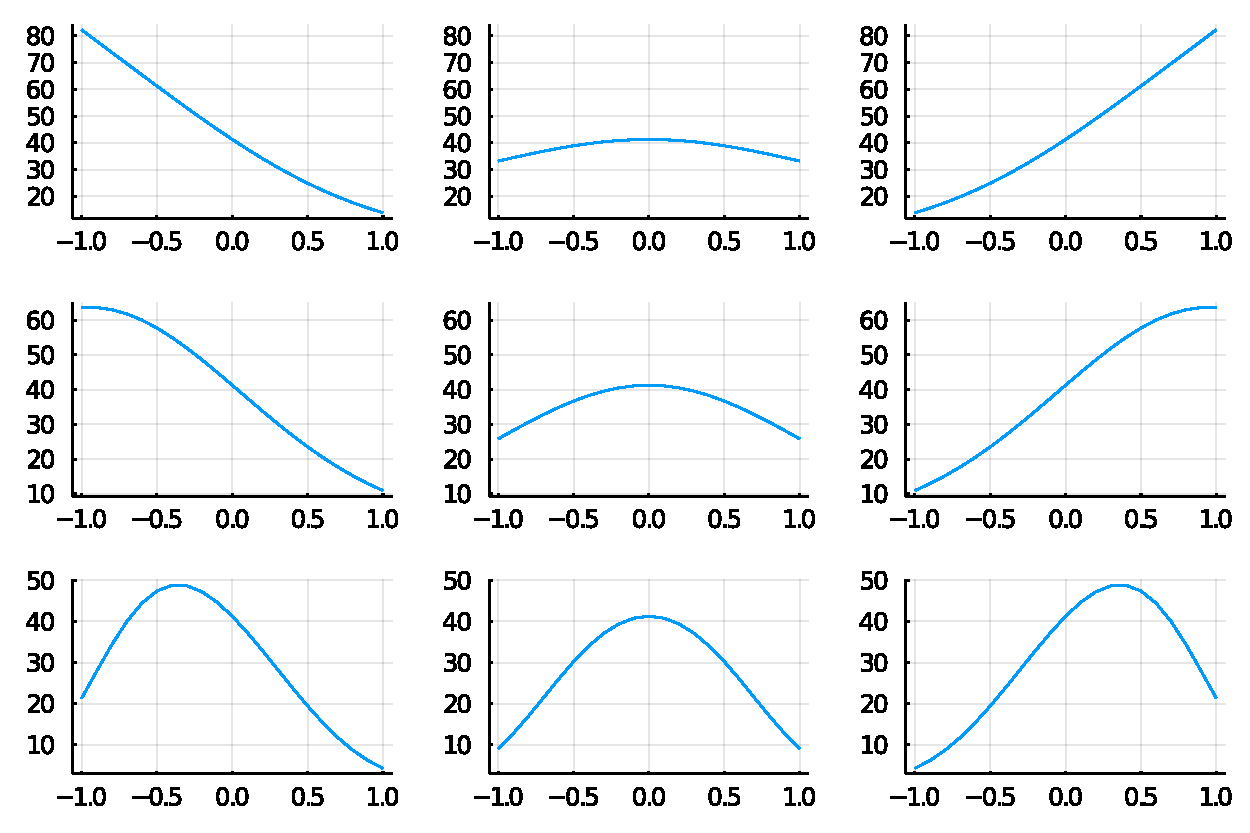
\includegraphics[width = \textwidth]{docs/Figures/Fig_Nsp_Temp.pdf}
    \caption{\textbf{\textit{Place holder:} The effects of variation in $E_a$ on the thermal sensitivity of species richness.} The relationship between species richness and temperature changes depending on the shape of the distribution of thermal sensitivities of interaction strengths, $E_a$. Plots show the shape of the N vs T relationship  }
    \label{fig:Nsp_Temp}
\end{figure}

\subsection{Assembly}

In order to test the bound on species richness we simulate the assembly of communities using the full GLV model in \cref{EQ:GLV}. Broadly we simulate assembly by starting with a small system ($N = 3$), allowing  and then sequentially invading 

randomly generate species with thermal sensitivity traits ($E$ and $B_0$s) for growth rates $r$ and interactions $a$ drawn from a global distribution. 

from a global distribution 

as follows . 

We simulate the assembly of communties as follows (see supplementary for full details). First we define the distribution of thermal response traits (the $B_0$ and $E$ values for growth and interactions) which for a given temperature allow us to calculate the distributions of growth rates and interaction strengths as outlined in \cref{SEC:Temperature}. These distributions of demographic parameters represent the traits of the global species pool, (i.e. the pool of potential invaders). Next we initialise the community by sampling from these distributions to generate a community with a small ($N=3$) number of species. We then simulate this community until the system reaches equilibrium, remove any extinct populations and add a new invader species at a low biomass with traits drawn from the distributions as described above. This process is repeated till a stable species richness is reached. An example of an assembly trajectory is shown in FIG. 

\section{Results}
\subsection{Analytical predictions of feasibility}

The feasibility bound show in in \cref{EQ:Feas_sp} 



\subsection{Temperature}

\subsubsection{Feasibility}

\subsubsection{Species Richness}

\subsection{Feasibility and Assembly}

\begin{figure}
    \centering
    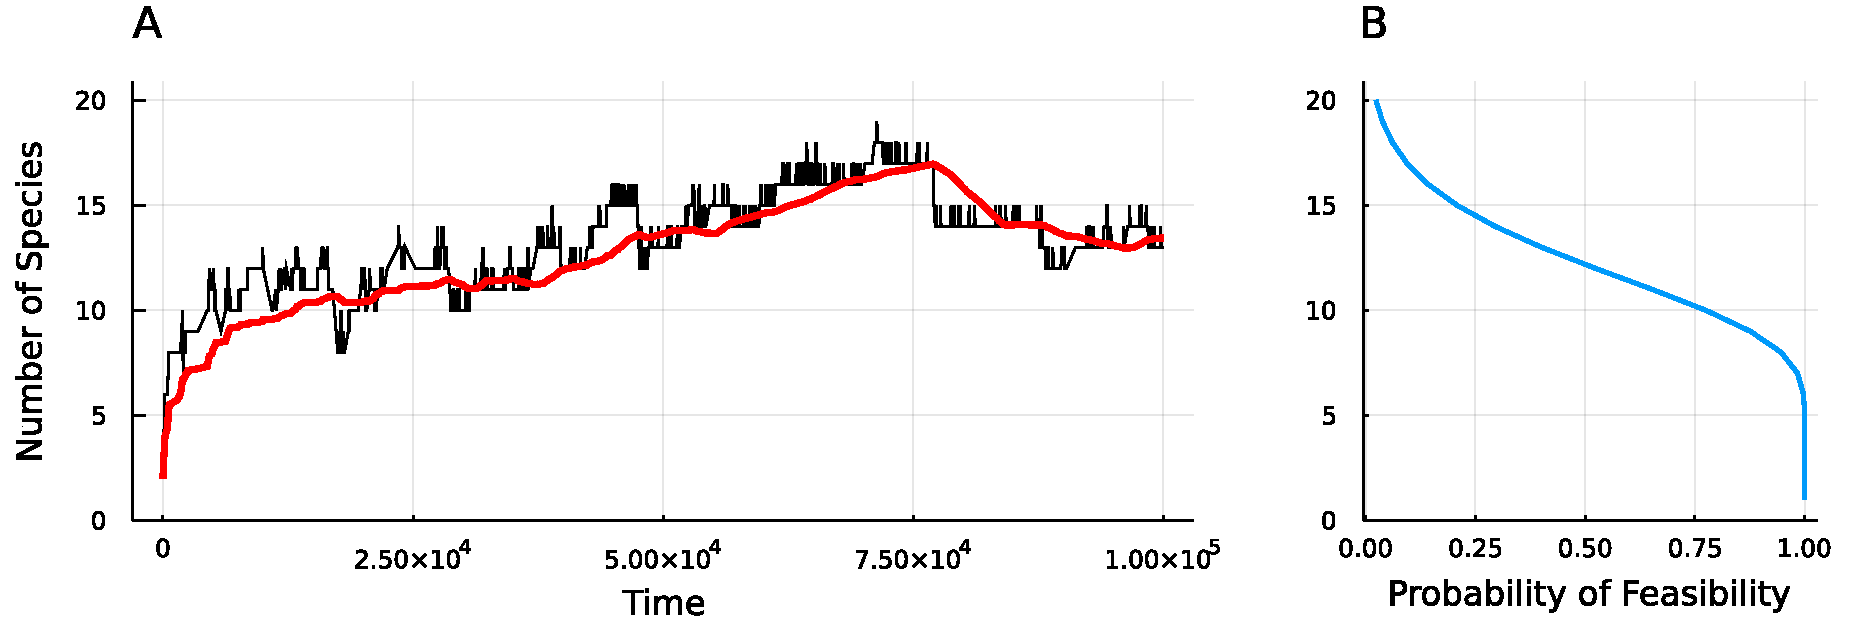
\includegraphics[width = \textwidth]{docs/Figures/Fig_3.pdf}
    \caption{Caption}
    \label{Fig:Assembly_Example}
\end{figure}


\begin{figure}
    \centering
    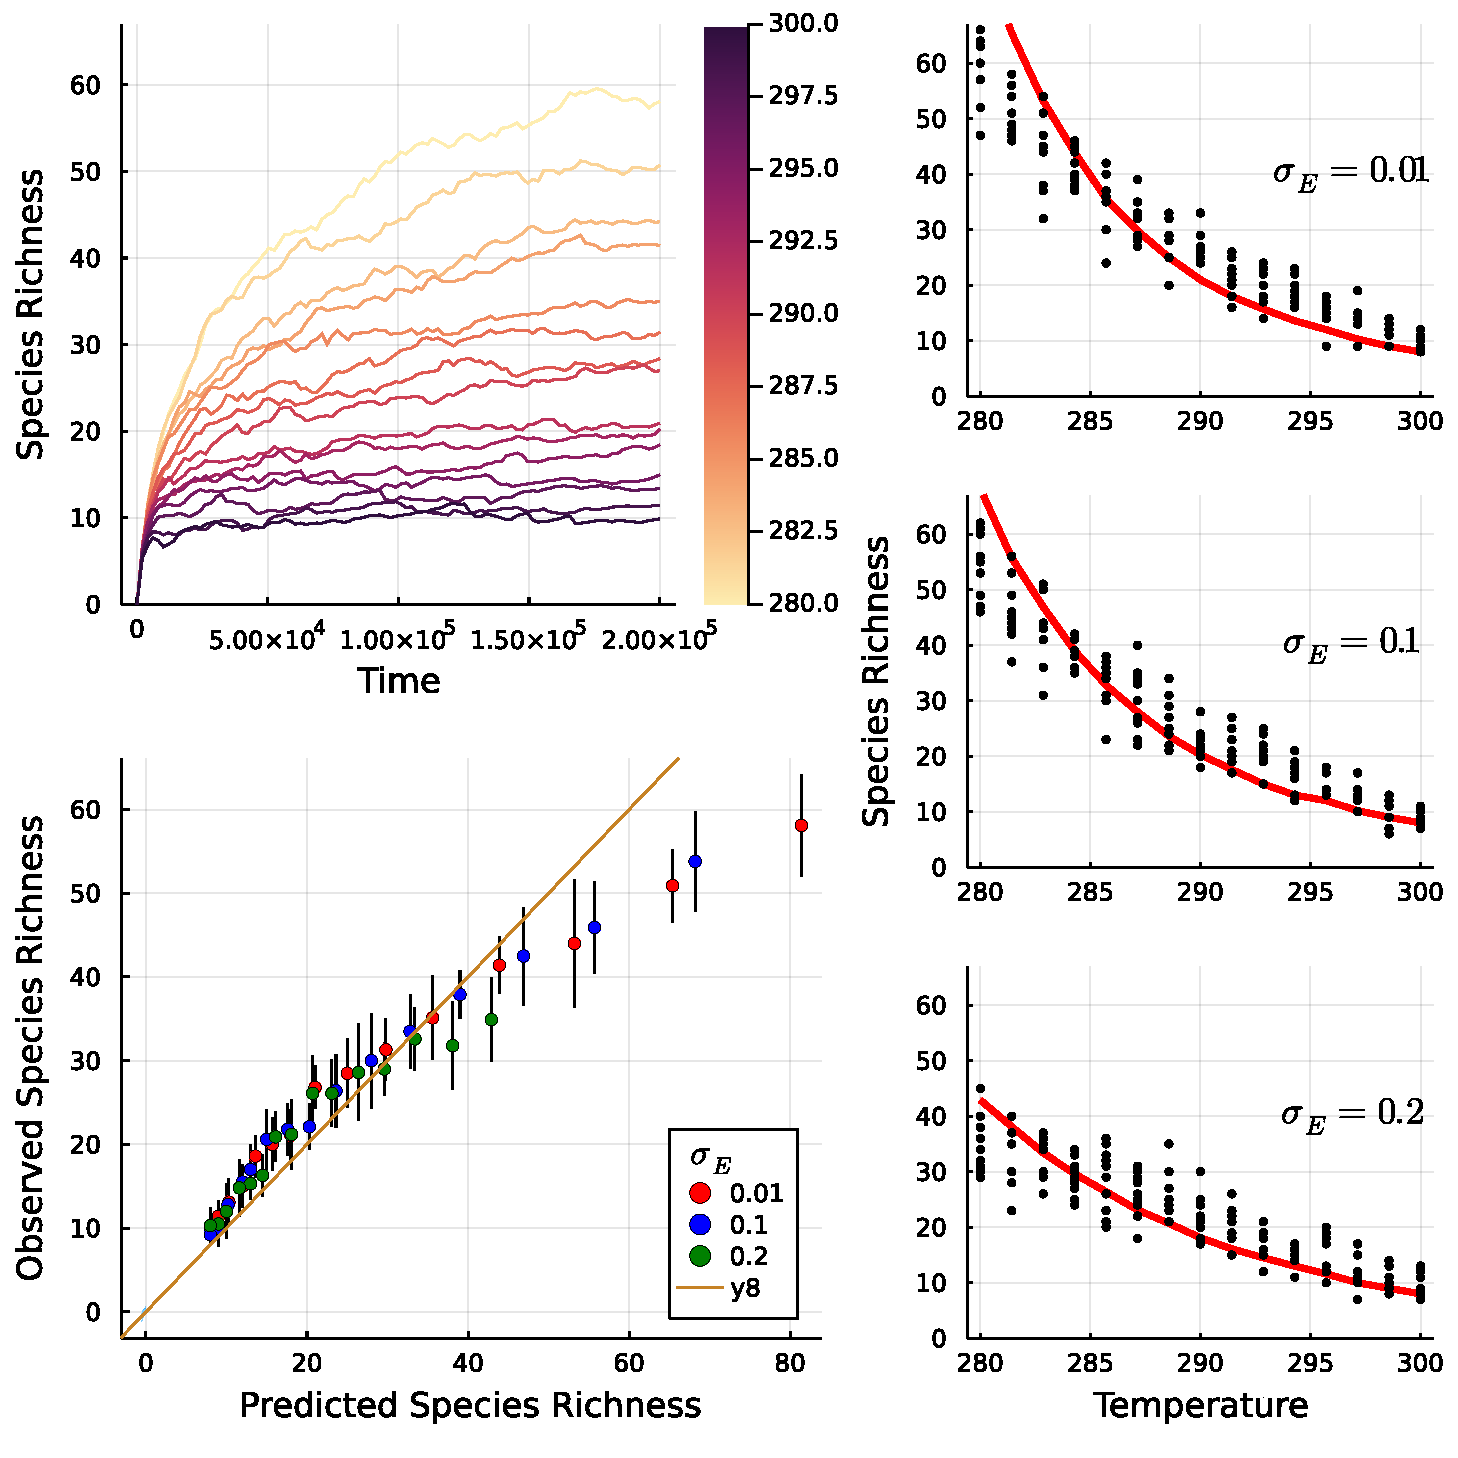
\includegraphics[width = \textwidth]{docs/Figures/Fig_4.pdf}
    \caption{Caption}
    \label{Fig:Temperature_assembly}
\end{figure}

\section{Supplementary Material}

\subsection{Mean-field approximation} \label{SI_Sec:Meanfield}

\subsection{Feasibility simulations} \label{SI_Sec:Feas_sims}

\subsection{Derivation of thermal response distributions} \label{SI_Sec:TPC_dist}


\end{document}
